Hubo using Hubo-Ach to walk and track a blue box.  
The robot will walk towards the blue box until it is within $0.2~m$ at which point it will stop.  
If the box moves, the robot will turn to track the box.
It is tracking the box in work-space via an RGBD camera and the HSV tracking method discribed in Section~\ref{sec:visTracking}.
Section~\ref{sec:walking:example} discribes the method used for the walking task.
Fig.~\ref{fig:visualSeroving} shows the robot completing this task.

\begin{figure}[thpb]
  \centering
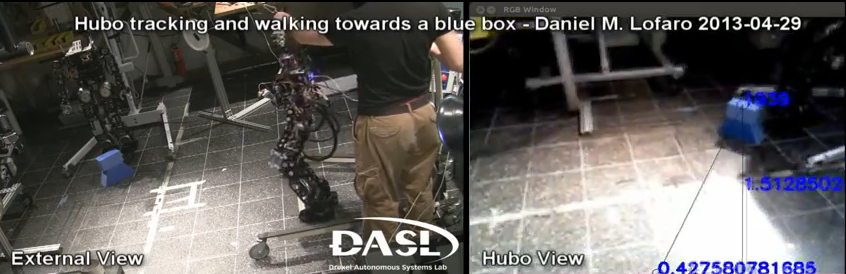
\includegraphics[width=0.79\columnwidth]{./pix/servoing.png}

\includegraphics[width=0.2\columnwidth]{./qrcode/qrcode-visualServoing.png}\\
     http://danlofaro.com/phd/tracking/\#TrackingAndWalking
  \caption{Hubo using Hubo-Ach to walk and track a blue box.  The robot will walk towards the blue box until it is within $0.2~m$ at which point it will stop.  If the box moves, the robot will turn to track the box.}
  \label{fig:visualSeroving}
\end{figure}
